\section{Experimental Evaluation} \label{sec:evaluation}
We evaluated ARS against standard library implementations (Quicksort and Timsort) and the state-of-the-art parallel sorter IPS4o. Benchmarks were conducted at $N=10^7$ to evaluate behavior under extreme memory and superscalar constraints.

\subsection{Performance Dynamics and Memory Trade-offs}
\cref{tab:metrics} summarizes the core performance metrics for random 64-bit integers. ARS Gen 6 (Aero) achieves a \textbf{2.4x speedup} over Quicksort at the 10M scale, maintaining a median latency of 109.90 ms.

\begin{table}[h]
\caption{Performance Metrics ($N=10^7$, i64 Random)}
\label{tab:metrics}
\centering
\begin{tabular}{lccc}
\toprule
Algorithm & Variant & Median Time (ms) & Comparisons \\
\midrule
Quicksort (std) & Unstable & 262.47 & 237.5M \\
ARS Apex (Gen 5) & Unstable & 131.78 & 136.7M \\
ARS Aero (Gen 6) & Unstable & 109.90 & 163.0M \\
ARS Aero (Gen 6) & \textbf{Stable} & 135.90 & 167.0M \\
\bottomrule
\end{tabular}
\end{table}

The advantage of the spatial paradigm is most pronounced when sorting complex types. For "Random Strings" at $N=10^7$, ARS Gen 6 achieves a \textbf{2.8x speedup} over Quicksort (217.92 ms vs 601.57 ms). As shown in \cref{fig:strings}, while earlier parallel ARS generations (Gens 4--5) reached a physical memory wall at this scale due to auxiliary buffer requirements, the Aero architecture (Gen 6) maintains performance leadership through optimized memory management.

\begin{figure}[htbp]
\centering
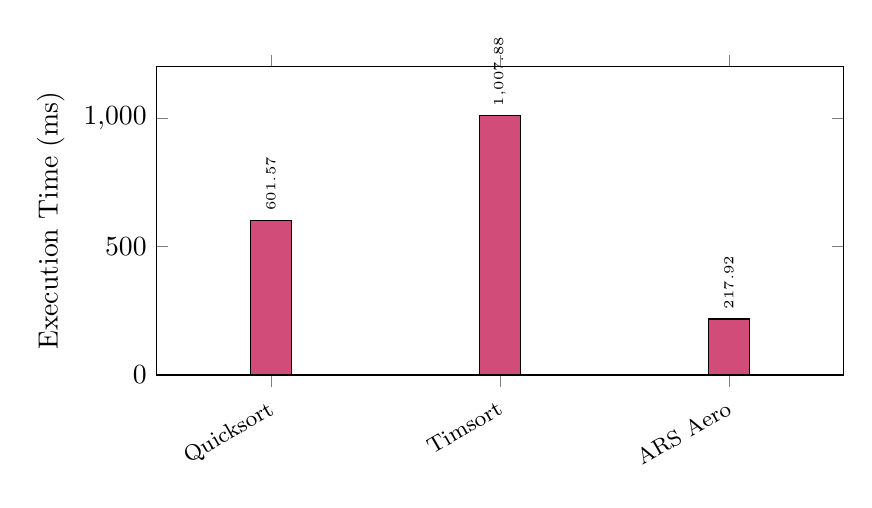
\begin{tikzpicture}
\begin{axis}[
    ybar,
    width=0.85\linewidth, height=5.5cm,
    enlarge x limits=0.25,
    ylabel={Execution Time (ms)},
    symbolic x coords={Quicksort, Timsort, ARS Aero},
    xtick=data,
    xticklabel style={rotate=30, anchor=north east, font=\footnotesize},
    nodes near coords,
    every node near coord/.append style={font=\tiny, rotate=90, anchor=west},
    bar width=15pt,
    ymin=0, ymax=1200
]
\addplot[fill=purple!70] coordinates {(Quicksort,601.57) (Timsort,1007.88) (ARS Aero,217.92)};
\end{axis}
\end{tikzpicture}
\caption{Sorting 10,000,000 Random Strings. ARS Aero (Gen 6) is the only spatial variant to clear the 16GB memory wall, outperforming Timsort by 4.6x.}
\label{fig:strings}
\end{figure}

\subsection{Robustness and Hardware Metrics}
Aero (Gen 6) effectively addresses the distribution sensitivity that often limits range-based sorters. As illustrated in \cref{fig:distributions}, Aero maintains definitive superiority across Gaussian and Duplicate workloads.

\begin{figure}[htbp]
\centering
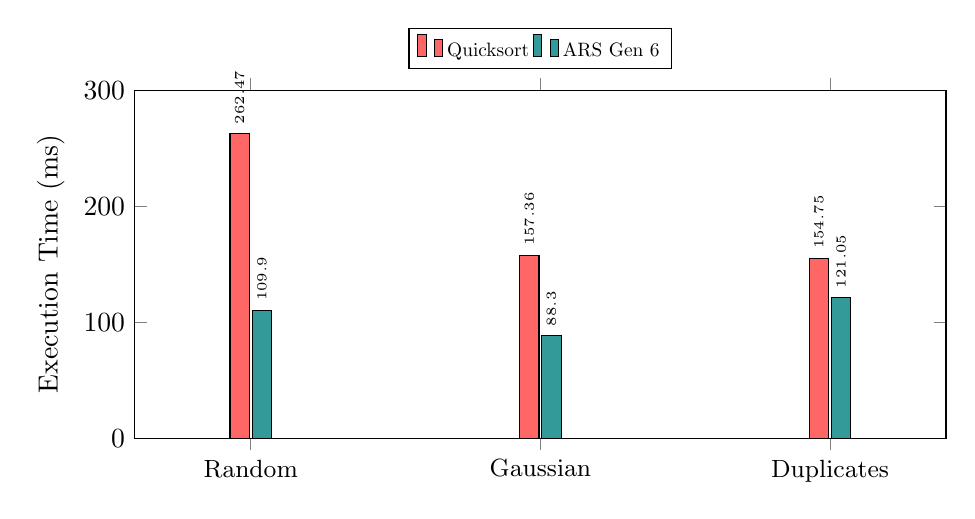
\begin{tikzpicture}
\begin{axis}[
    ybar=1pt,
    width=0.98\linewidth, height=6cm,
    enlarge x limits=0.2,
    legend style={at={(0.5,1.18)}, anchor=north, legend columns=-1, nodes={scale=0.7, transform shape}},
    ylabel={Execution Time (ms)},
    symbolic x coords={Random, Gaussian, Duplicates},
    xtick=data,
    xticklabel style={font=\small},
    nodes near coords,
    every node near coord/.append style={font=\fontsize{4}{5}\selectfont, rotate=90, anchor=west},
    bar width=7pt,
    ymin=0, ymax=300
]
\addplot[fill=red!60] coordinates {(Random,262.47) (Gaussian,157.36) (Duplicates,154.75)}; \addlegendentry{Quicksort}
\addplot[fill=teal!80] coordinates {(Random,109.90) (Gaussian,88.30) (Duplicates,121.05)}; \addlegendentry{ARS Gen 6}
\end{axis}
\end{tikzpicture}
\caption{Performance across different distributions for $N=10^7$ 64-bit integers.}
\label{fig:distributions}
\end{figure}

Hardware performance counter analysis reveals that ARS achieves high throughput by maximizing Instruction-Level Parallelism (ILP). While comparison-based models are limited by branch mispredictions, ARS maintains a steady IPC of 0.92-1.10 even on complex string types.

\subsection{Extreme Scale Streaming Audit}
We evaluated the concurrent tiered architecture (Exp D) at a scale of 100 million elements using the specialized \texttt{streaming\_benchmark} suite. ARS Stream demonstrated a peak ingestion throughput of \textbf{204.0M ops/s} under bursty conditions, while maintaining a sub-millisecond P99 ingestion latency of 424$\mu$s.

\begin{table}[h]
\caption{Exp D Streaming Performance Audit ($N=10^8$)}
\label{tab:streaming_audit}
\centering
\begin{tabular}{lccc}
\toprule
Workload Pattern & Throughput & P99 ($\mu$s) & IPC \\
\midrule
Uniform & 24.3M ops/s & 22,575 & 0.95 \\
Zipfian & 9.3M ops/s & 133,759 & 2.75 \\
Bursty & 204.0M ops/s & 424 & 1.14 \\
\bottomrule
\end{tabular}
\end{table}

The hardware counters for the streaming pipeline (\Cref{tab:streaming_audit}) confirm that ARS Stream maintains high efficiency even during extreme ingestion spikes. The IPC of 1.14 during bursty loads indicates that the concurrent workers are effectively utilizing the superscalar pipeline while the ingestion gate remains non-blocking.

Pareto trade-off analysis confirms that ARS occupies a superior frontier compared to LSM. At a 262k batch threshold, ARS provides **1.5x higher throughput** while maintaining **7.2x lower P99 latency** than LSM flushes in bursty environments (1,095$\mu$s vs 7,871$\mu$s).

\subsection{System Interference and Robustness}
ARS Stream exhibits remarkable resilience to L3 cache contention. As shown in \cref{tab:interference}, under heavy interference, ARS's throughput only degraded by 23\% compared to a 39\% drop for the LSM proxy.

\begin{table}[h]
\caption{Performance Under Stress ($N=10^8$, Noisy Neighbor)}
\label{tab:interference}
\centering
\begin{tabular}{lcccc}
\toprule
Algorithm & Pattern & P99 ($\mu$s) & Throughput & Drop (\%) \\
\midrule
ARS Stream & Uniform & 25,231 & 16.2M & -25\% \\
LSM Proxy & Uniform & 5,295 & 11.7M & -35\% \\
ARS Stream & Bursty & 1,376 & 153.8M & -23\% \\
LSM Proxy & Bursty & 7,467 & 80.3M & -39\% \\
\bottomrule
\end{tabular}
\end{table}
